% Short paper for Optimization Letters.
% Compile: pdflatex -> bibtex -> pdflatex x2
% Springer's sn-jnl.cls is not bundled here; `article` + natbib compiles anywhere
% and the content maps onto the OL template without change.
\documentclass[11pt,a4paper]{article}
\usepackage[margin=1in]{geometry}
\usepackage{amsmath,amssymb,booktabs,graphicx,microtype}
\usepackage[round]{natbib}
\usepackage[hidelinks]{hyperref}
\graphicspath{{figures/}}

\title{Restarts substitute for initialization in the Nelder--Mead method,\\
       and which restart trigger wins depends on dimension}

% AFFILIATION PENDING -- to be supplied by the author.
% Note for submission: the CAPES transformative agreement requires the
% *corresponding* author to be affiliated with a participating Brazilian
% institution at the time of acceptance. Set this before submitting.
\author{%
  Marco Mollinetti\\
  \small\textit{[affiliation to be supplied]}
}
\date{}

\begin{document}
\maketitle

\begin{abstract}
\citet{wessing2019} showed that the initial simplex changes Nelder--Mead's
runtime by orders of magnitude, and that the effect survives Kelley's oriented
restarts. That robustness check held the restart scheme fixed, so the
interaction was never quantified. We cross seven initialization procedures with
six restart triggers and two restart constructions on the COCO/BBOB noiseless
suite at $n\in\{2,5,10,20\}$ ($43\,050$ runs). Restarts largely substitute for
initialization: the spread in initializer mean rank falls from $2.68$ under a
single descent to $0.89$--$1.24$ once a trigger is enabled, and the MATLAB
\texttt{fminsearch} initializer---worst of seven under a single descent---becomes
unremarkable. The substitution erodes with dimension, the spread under a working
trigger rising from $0.34$ at $n=2$ to $2.26$ at $n=20$. Turning to the trigger
itself, we find the choice is strongly dimension-dependent, and the two
published detectors sit at opposite ends of that dependence. The
simplex-degeneracy test of \citet{luersen2004} degrades monotonically---from
$74.5\%$ of problems solved at $n=2$ to $4.2\%$ at $n=20$, against $11.4\%$ for
not restarting at all---while accounting for a rising share of all firings,
$60.7\%$ at $n=2$ to $100\%$ at $n=20$, and thrashing at $463$ restarts per run.
A sweep of its two tolerances over $40$ orders of magnitude shows the second of
these is a mis-setting rather than a property of the criterion---retuning cuts
the restart rate at $n=20$ from $442$ to $13$---but that no setting makes the
criterion better than a plain simplex-size test at any dimension, and that its
edge-ratio tolerance is inert in $11$ of the $12$ cells tested.
The sufficient-decrease test of \citet{kelley1999} moves the other way, from
$5.5$ points \emph{below} the no-restart baseline at $n=2$ to $15.0$ points above
it at $n=20$: it is the only trigger whose advantage grows with dimension
(Cochran--Armitage $p=9.1\times10^{-6}$, though the point comparison at $n=20$
alone does not survive correction for multiplicity). Two
trivial triggers---restart when the simplex is small, or when its vertex values
are flat---are the most reliable across the range. Conditioning, the obvious
mechanism, does not mediate any of this ($\rho\approx-0.05$), and the unshifted
analytic functions still standard in this literature reverse the substitution
result entirely.
\end{abstract}

\noindent\textbf{Keywords:} Nelder--Mead $\cdot$ direct search $\cdot$ simplex
initialization $\cdot$ restart strategies $\cdot$ derivative-free optimization
$\cdot$ benchmarking

\section{Introduction}

The Nelder--Mead simplex method \citep{nelder1965} remains among the most widely
used derivative-free optimizers despite the absence of general convergence
guarantees \citep{mckinnon1998,lagarias1998}. Two design choices govern its
practical behaviour, and the literature has treated them separately.

The first is the initial simplex. \citet{wessing2019} showed that common
initialization procedures inflate runtime by orders of magnitude even on a
spherical objective, and recommended normalizing the search space and choosing
the simplex independently of the starting point. \citet{takenaga2023} studied
initial simplex size and shape under a limited evaluation budget;
\citet{han2006} examined the interaction with dimension.

The second is the restart policy, and in particular its \emph{trigger}: the test
that decides the method has stopped making progress. \citet{kelley1999} detects
stagnation by failure of a sufficient-decrease condition on the mean vertex
value and remedies it with an oriented restart. \citet{luersen2004} restart on
simplex smallness, on flatness of the vertex values, or on simplex
\emph{degeneracy}. \citet{hansen2009nm} benchmarked a two-level restart schedule
and \citet{posik2012} compared restarted local searchers, Nelder--Mead among
them.

These literatures do not meet. Wessing ran his comparison against Kelley's
restarting variant, but as a robustness check: the restart scheme was fixed and
the interaction was not measured. Nor, to our knowledge, has any trigger been
ablated against the others. Both detectors above are motivated---one by a
descent argument, one by simplex geometry---and neither has been compared to the
trivial alternative of restarting when the simplex simply becomes small. We ask:

\begin{quote}
\textbf{(Q1)} Do restarts substitute for initialization---and over what
dimension?

\textbf{(Q2)} Which trigger should fire the restart, and do the principled
detectors earn their complexity?
\end{quote}

Section~\ref{sec:design} describes a factorial answering both. Because trigger
and re-seeding are easy to confound---Kelley's detector is published together
with a deliberately \emph{local} re-seed, while the others are naturally paired
with a global one---we vary restart construction as a third factor rather than
assuming it away.

\section{Background: the two detectors}
\label{sec:background}

Let $S^k$ have vertices ordered by objective value, let $D^k f$ denote the
simplex gradient, and let
\[
  L(Y) = \bigl[\, y^1-y^0,\dots,y^n-y^0 \,\bigr] = \bigl[\,e^1,\dots,e^n\,\bigr]
\]
be the edge matrix, with $\sigma_+$ and $\sigma_-$ the largest and smallest edge
length.

\paragraph{Kelley's sufficient-decrease test.}
\citet{kelley1999} flags stagnation when the $k+1$st iteration fails
\begin{equation}
  \bar f^{\,k+1} - \bar f^{\,k} < -\alpha \lVert D^k f\rVert^2 ,
  \label{eq:kelley}
\end{equation}
where $\bar f$ is the \emph{mean} of the vertex values---not the best, which a
Nelder--Mead iteration is not guaranteed to improve---and
$\alpha = \alpha_0\,\sigma_+(S^0)/\lVert D^0 f\rVert$. A restart is performed
when \eqref{eq:kelley} fails but $\bar f^{\,k+1}-\bar f^{\,k}<0$. The remedy is
an \emph{oriented restart}: a smaller simplex with orthogonal edges of length
$\tfrac12\sigma_-(S^k)$ aligned against the sign pattern of $D^k f$.

\paragraph{GBNM's degeneracy test.}
The globalized bounded Nelder--Mead of \citet{luersen2004} declares a simplex
degenerate---and reinitializes it---when it is neither small nor on a bound and
\begin{equation}
  \frac{\min_k \lVert e^k\rVert}{\max_k \lVert e^k\rVert} < \varepsilon_{s3}
  \qquad\text{or}\qquad
  \frac{\lvert \det L(Y)\rvert}{\prod_k \lVert e^k\rVert} < \varepsilon_{s4}.
  \label{eq:gbnm9}
\end{equation}
The second quantity is the Hadamard ratio, equal to $1$ for orthogonal edges and
$0$ for linearly dependent ones, independently of length. Both are translation-
and scale-invariant, which is what makes them usable as a shape diagnostic.
Equation~\eqref{eq:gbnm9} is thus a conditioning-triggered restart, predating the
geometry-driven model-improvement steps of model-based derivative-free
optimization \citep{conn2009}. Related ideas constrain the \emph{operations}
instead: \citet{tseng2000} and \citet{nazareth2002} hold the simplex volume above
a threshold so interior angles stay bounded away from zero.

A separate line restores convergence by constraining the simplex directly rather
than restarting it: \citet{price2002} poll a positive basis, \citet{burmen2006}
restrain the simplex to a grid, and \citet{gao2012} adapt the coefficients to
dimension---the second variant on which \citet{wessing2019} confirmed his
initialization effect. Coefficient choice has been revisited since
\citet{barton1996}, and \citet{wang2011} give a parameter sensitivity study of
the method---but of the reflection, expansion and contraction coefficients and
the initial simplex size, not of any restart tolerance. None treat the trigger as
the object of study.

Luersen and Le Riche report that $\varepsilon_{s3}$ and $\varepsilon_{s4}$ ``may
be difficult to tune, so that a simplex which is becoming small may be tagged as
degenerated before,'' and add a rule requiring two consecutive detections to
compensate; the same machinery carries into their constrained variant
\citep{luersen2004smo}. That admission appears not to have been followed up.

\section{Experimental design}
\label{sec:design}

\paragraph{Factor A: initialization (7 levels).}
\texttt{pfeffer}, the MATLAB \texttt{fminsearch} default and the principal
subject of \citet{wessing2019}; the regular simplex of \citet{spendley1962},
which is also GBNM's Eq.~(A.1), at edge scales of $100\%$, $10\%$ and $2\%$ of
the smallest box dimension, the latter two spanning the range from which GBNM
draws restart simplices; \texttt{uniform} and \texttt{gaussian} random
simplices; and a minimal positive spanning basis $W=ZB^{-}$.

\paragraph{Factor B: restart trigger (6 levels).}
The six below are the triggers in current use. One classical alternative is not
included: the factorial test of \citet{oneill1971}, which perturbs each
coordinate at the converged point to check it is a local minimum and restarts if
it is not. It costs $2n$ evaluations per invocation rather than none, which puts
it in a different class from the six here, and we leave it to future work.
\texttt{none} (single descent, terminated rather than restarted); \texttt{size}
(small simplex); \texttt{flat} (small spread of vertex values);
\texttt{conditioning} (Eq.~\eqref{eq:gbnm9}); \texttt{gbnm} (size $\lor$
conditioning, as published); and \texttt{progress} (Eq.~\eqref{eq:kelley}).

\paragraph{Factor C: restart construction (2 levels).}
\texttt{gaussian\_best}, a fresh simplex drawn about the incumbent---a global
move on a bounded box; and \texttt{oriented}, Kelley's Eq.~(8.7)---a deliberately
local move. \texttt{none} takes no construction and \texttt{progress} appears
only in its published pairing, giving $7\times(1+1+4\times2)=70$ arms.

\paragraph{Benchmark.}
COCO/BBOB noiseless \citep{hansen2021coco}, $f_1$--$f_{24}$,
$n\in\{2,5,10,20\}$, instances $1$--$5$: $480$ problems $\times$ $70$ arms
$=33\,600$ runs at a budget of $2000n$ evaluations. BBOB shifts and rotates each
instance, so a structured simplex centred in the box gains no unearned
advantage. This COCO build does not expose $f_{\mathrm{opt}}$, so the reference
is $f_L$, the best value reached by any arm, and the convergence test is that of
\citet{more2009}, $f(x_0)-f(x)\ge(1-\tau)(f(x_0)-f_L)$, at
$\tau\in\{10^{-1},10^{-3},10^{-5},10^{-7}\}$; this is the budget-aware
alternative to the performance profiles of \citet{dolan2002}. We additionally
ran the same factorial on five unshifted analytic functions at
$n\in\{2,5,10\}$ ($15$ seeds; $9450$ runs), not as evidence but as a control on
the benchmark itself. The control does not extend to $n=20$, so the comparison in
Section~\ref{sec:caution} is drawn over three dimensions rather than four.

\paragraph{Reporting rule.}
Results are reported per dimension. We pool across dimensions \emph{only where
the ordering is dimension-stable}, and say so at each point; the central finding
below is that for several comparisons it is not, and a pooled number would then
be an artifact of which dimensions happened to be run.

\paragraph{Statistical protocol.}
The unit of analysis is the \emph{problem}, not the run: the seven initializers
on one problem are not independent, so each problem is reduced to a single
outcome (solved by a majority of the seven) before any test. Paired comparisons
use an exact McNemar test on those outcomes, and Holm correction is applied
across the entire family of $32$ comparisons the paper reads, so no claim below
rests on an uncorrected $p$-value. Effect sizes are reported as the paired win
rate $P(\text{arm A ends lower}\mid\text{same problem})$, read on the
conventional $0.56/0.64/0.71$ small/medium/large scale.

Two choices deserve a word. We do not use a Wilcoxon signed-rank on the raw
objectives: BBOB values carry per-instance offsets and span many orders of
magnitude, so that test is dominated by whichever problems happen to have large
$|f|$. And we do not use the unpaired Vargha--Delaney $A_{12}$, which across all
cross-pairs compares one arm on one problem against another arm on a different
problem; problem difficulty then swamps the arm effect, and it returns
``negligible'' for comparisons whose paired win rates run from $20\%$ to $97\%$.

Finally, the paper's dimensional claims are claims about a \emph{trend}, and
testing them as four separate point comparisons is both the wrong question and
needlessly weak. We test them directly with a Cochran--Armitage trend test on the
share of discordant pairs, with $\log_2 n$ as the dose.

\paragraph{Response.}
Besides solved fractions we log, per iteration, both quantities of
Eq.~\eqref{eq:gbnm9} and which criterion fired at each restart. The Hadamard
ratio is computed in log space via a signed log-determinant; evaluated directly
it underflows to \texttt{NaN} at $n=10$ once edge lengths reach $10^{-40}$, that
is, exactly in the degenerate regime of interest.

\section{Results}
\label{sec:results}

\subsection{The best trigger depends on the dimension}
\label{sec:ablation}

\begin{figure}[t]
\centering
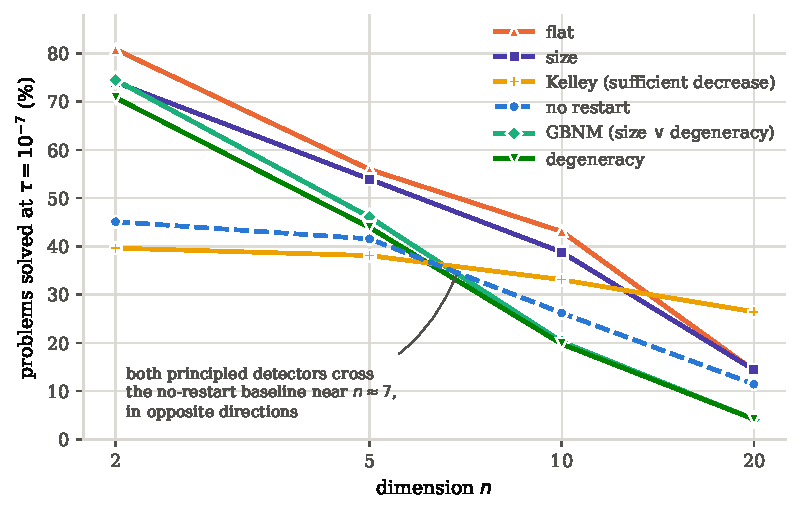
\includegraphics[width=0.78\textwidth]{fig1-triggers.pdf}
\caption{Problems solved at $\tau=10^{-7}$ against dimension, at
\texttt{gaussian\_best} construction (\texttt{progress} in its published
pairing). The two principled detectors cross the no-restart baseline near
$n\approx7$ in \emph{opposite} directions.}
\label{fig:triggers}
\end{figure}

\begin{table}[t]
\centering
\caption{Problems solved at $\tau=10^{-7}$ (\%) and restarts per run, by
dimension. Constructions are \texttt{gaussian\_best} except \texttt{progress},
which appears in its published pairing with \texttt{oriented}.}
\label{tab:triggers}
\small
\begin{tabular}{lcccc c cccc}
\toprule
& \multicolumn{4}{c}{solved at $\tau=10^{-7}$ (\%)} && \multicolumn{4}{c}{restarts per run} \\
\cmidrule(lr){2-5}\cmidrule(lr){7-10}
trigger & $n{=}2$ & $n{=}5$ & $n{=}10$ & $n{=}20$ && $n{=}2$ & $n{=}5$ & $n{=}10$ & $n{=}20$ \\
\midrule
\texttt{flat}          & \textbf{80.8} & \textbf{56.0} & \textbf{43.1} & 14.3 && 53.8 & 40.9 & 27.3 & 11.8 \\
\texttt{size}          & 74.0 & 53.9 & 38.8 & \textbf{14.4} && 33.7 & 28.0 & 18.0 & 7.3 \\
\texttt{gbnm}          & 74.5 & 46.1 & 20.2 & 4.2 && 79.9 & 93.5 & 131.1 & 463.3 \\
\texttt{conditioning}  & 70.8 & 43.9 & 19.8 & 4.2 && 64.0 & 86.7 & 126.4 & 462.5 \\
\texttt{progress}      & 39.6 & 38.1 & 33.1 & \textbf{26.4} && 7.5 & 23.9 & 20.4 & 22.4 \\
\texttt{none}          & 45.1 & 41.5 & 26.2 & 11.4 && 0 & 0 & 0 & 0 \\
\bottomrule
\end{tabular}
\end{table}

Figure~\ref{fig:triggers} and Table~\ref{tab:triggers} carry the paper's main
result: \emph{the ranking of restart triggers is not stable across dimension},
and the two published detectors sit at opposite ends of that instability.

The degeneracy test degrades monotonically, from $74.5\%$ at $n=2$ to $4.2\%$ at
$n=20$. It starts above the no-restart baseline and ends far below it: at $n=10$
it solves $20.2\%$ against the baseline's $26.2\%$, and at $n=20$ it solves
$4.2\%$ against $11.4\%$---roughly a third as many problems as never restarting.
Kelley's detector moves the other way, from $5.5$ points below the baseline at
$n=2$ to $15.0$ points above it at $n=20$. It is the only trigger whose
advantage over not restarting grows with dimension, and the two cross the
baseline in opposite directions at nearly the same place, $n\approx7$.

Both trends are significant when tested as trends. The share of
discordant problems favouring Kelley over no-restart rises $0.00 \to 0.18 \to
0.54 \to 0.77$ across the four dimensions (Cochran--Armitage $z=+4.44$,
$p=9.1\times10^{-6}$), while for the degeneracy trigger it falls $1.00 \to 0.55
\to 0.06 \to 0.00$ ($z=-7.80$, $p=6.0\times10^{-15}$). Read instead as point
comparisons, the picture is more uneven and we report it as such: the degeneracy
trigger is significantly worse than no-restart at $n=10$ and $n=20$ after Holm
correction ($p=9.3\times10^{-3}$ and $3.5\times10^{-4}$; at $n=20$ it solves
\emph{no} problem that no-restart misses, against $17$ the other way), whereas
Kelley's advantage at $n=20$ does \emph{not} survive correction as an isolated
comparison ($p=0.094$). The Kelley result is therefore a trend claim, and we make
it only as one.

The two trivial triggers are the most reliable across the range, and both
beat both principled detectors at every dimension from $n=5$ upward. We do not
rank them against each other: \texttt{flat} leads on the relative measure at
$n\le10$ and \texttt{size} on the absolute one at $n=10$, and a paired test
separates them only at $n=2$ (in \texttt{flat}'s favour, $p=1.6\times10^{-3}$);
everywhere else they are indistinguishable. At $n=2$
\texttt{gbnm} and \texttt{size} are indistinguishable ($74.5$ vs.\ $74.0$), so
the advantage of the trivial triggers is a claim about $n\ge5$, not about the
whole range. Since that ordering \emph{is} dimension-stable over $n\ge5$, we
state it pooled: adding Eq.~\eqref{eq:gbnm9} to a size test makes the
combination worse, which is stronger than the test merely failing to help. That
comparison survives correction at every dimension from $n=5$ ($p\le2.7\times
10^{-2}$), with paired win rates of $0.650$, $0.633$ and $0.692$---a medium
effect. The corresponding comparison against no-restart is large at every
dimension ($0.771$ to $0.979$).

Varying construction does not change these conclusions. Under \texttt{oriented}
re-seeding the trivial triggers still lead at $n\le10$ ($47.4$--$50.1\%$ against
$31.9$--$48.5\%$), and construction has a large main effect of its own---the
local re-seed costs every trigger $11.5$ to $16.7$ points pooled---but it does
not reorder the triggers except at $n=20$, where all four fall within a point of
each other ($12.1$--$12.9\%$) and the comparison carries no information.

\subsection{Why the degeneracy trigger collapses}
\label{sec:degeneracy}

\begin{figure}[t]
\centering
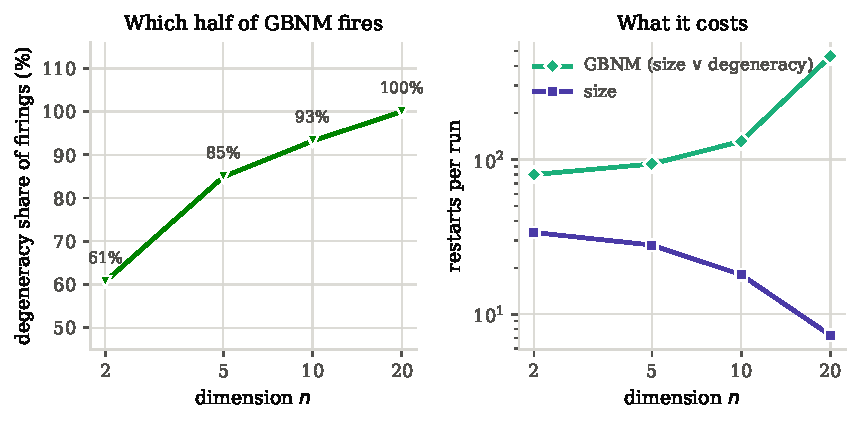
\includegraphics[width=0.84\textwidth]{fig2-gbnm.pdf}
\caption{Left: the share of GBNM restarts fired by the degeneracy half of
Eq.~\eqref{eq:gbnm9} rather than the size half. Right: what that costs. As
dimension grows GBNM becomes its degeneracy test, and that test thrashes.}
\label{fig:gbnm}
\end{figure}

Figure~\ref{fig:gbnm} explains the collapse and vindicates the concern of
\citet{luersen2004} about their tolerances. Under the combined trigger the share
of restarts fired by the degeneracy test rather than the size test rises from
$60.7\%$ at $n=2$ to $84.9\%$, $93.2\%$ and finally $100.0\%$ at $n=20$: at that
dimension GBNM \emph{is} its degeneracy test, the size half never firing at all.
Meanwhile the cost diverges. The degeneracy trigger fires $463$ times per run at
$n=20$ against $7.3$ for a size test---a $63$-fold difference, in the direction
of the worse method. Each restart discards the current simplex, so the method
spends its budget rebuilding rather than descending.

This is the failure mode Luersen and Le Riche anticipated: a shrinking simplex
is tagged degenerate before it is tagged small. Their two-consecutive-detections
rule mitigates a problem whose magnitude, as far as we can determine, has not
previously been measured, and which grows without bound in dimension.

\subsection{Is the failure a tuning artifact? A calibration of $\varepsilon_{s3}$ and $\varepsilon_{s4}$}
\label{sec:calibration}

The indictment in Section~\ref{sec:degeneracy} is only worth making if the
failure belongs to the criterion rather than to the tolerances we happened to
run it at---the more so because its authors call those tolerances hard to tune.
We therefore swept both, log-spaced from fully disabled to maximally aggressive,
holding the initializer at the regular simplex and comparing against a plain
size test in the same harness. The response is the fraction of problems on which
the degeneracy arm ends lower than the size arm; $50\%$ is parity. Table~\ref{tab:calibration}
reports it, with the resulting restart rate alongside.

\begin{table}[t]
\centering
\caption{Tolerance calibration. Win rate against a size test (\% of problems
where the degeneracy trigger ends lower; $50\%$ = parity) and restarts per run.
$\varepsilon_{s3}$ is held at $10^{-12}$: it is inert in $11$ of $12$ cells (see
text), so the table is indexed by $\varepsilon_{s4}$ alone.}
\label{tab:calibration}
\small
\begin{tabular}{rcc cc cc}
\toprule
& \multicolumn{2}{c}{$n=5$} & \multicolumn{2}{c}{$n=10$} & \multicolumn{2}{c}{$n=20$} \\
\cmidrule(lr){2-3}\cmidrule(lr){4-5}\cmidrule(lr){6-7}
$\varepsilon_{s4}$ & win & restarts & win & restarts & win & restarts \\
\midrule
$0$ (disabled) & 15.0\% & 0 & 20.8\% & 0 & 15.8\% & 0 \\
$10^{-40}$ & 33.3\% & 58.1 & 39.2\% & 11.9 & \textbf{54.2\%} & 13.0 \\
$10^{-20}$ & 30.8\% & 60.7 & \textbf{44.2\%} & 18.3 & 42.5\% & 44.8 \\
$10^{-12}$ & 31.7\% & 66.4 & 37.5\% & 39.4 & 27.5\% & 111.1 \\
$10^{-6}$ (default) & 27.5\% & 86.3 & 40.8\% & 122.1 & 20.0\% & 442.5 \\
$10^{-4}$ & 28.3\% & 114.7 & 35.0\% & 238.4 & 10.0\% & 1669.2 \\
$10^{-2}$ & 28.3\% & 252.9 & 20.8\% & 1148.5 & 10.0\% & 1904.0 \\
\bottomrule
\end{tabular}
\end{table}

Three things follow.

\paragraph{$\varepsilon_{s3}$ does almost nothing.} Across four orders of
magnitude, $10^{-12}$ to $10^{-2}$, the edge-ratio half of Eq.~\eqref{eq:gbnm9}
leaves both the win rate and the restart rate unchanged in $11$ of the $12$
(dimension, $\varepsilon_{s4}$) combinations tested, to the digits shown. The
single exception is $n=5$ at $\varepsilon_{s4}=10^{-12}$, where loosening
$\varepsilon_{s3}$ to $10^{-2}$ moves the win rate from $31.7\%$ to $27.5\%$;
at $n=10$ and $n=20$ it is inert everywhere. The Hadamard half does essentially
all the work, so in practice GBNM's two tolerances are one knob---worth knowing
for anyone trying to tune it. Table~\ref{tab:calibration} is therefore indexed
by $\varepsilon_{s4}$ alone, at $\varepsilon_{s3}=10^{-12}$.

\paragraph{The default is badly mis-set at high dimension.} Moving
$\varepsilon_{s4}$ from the default $10^{-6}$ down to $10^{-40}$ raises the win
rate at $n=20$ from $20.0\%$ to $54.2\%$---$34$ points---and cuts the restart
rate from $442$ per run to $13$. The trigger is not inherently a thrashing
mechanism; it is a correctly-shaped criterion set thirty orders of magnitude too
loose for a degenerating simplex, whose Hadamard ratio routinely reaches
$10^{-40}$. This is the effect Luersen and Le Riche describe qualitatively.

\paragraph{But no setting makes it worth having.} Testing all $21$ cells against
parity with a two-sided binomial test and a Bonferroni correction
($\alpha=0.05/21$), \emph{none} is significantly better than a plain size test at
any dimension. The single above-parity cell---$n=20$ at $\varepsilon_{s4}=10^{-40}$,
$54.2\%$---has $p=0.41$ and is indistinguishable from a coin flip. Eleven of the
$21$ cells are significantly \emph{worse}. Disabling the criterion outright is
worse still ($15$--$21\%$), so restarting does useful work; it is the degeneracy
criterion specifically that adds nothing a size test does not already provide.

The conclusion of Section~\ref{sec:degeneracy} therefore survives, but its scope
changes. ``Actively harmful'' is a statement about the published default, not
about the criterion: correctly tuned, the trigger is merely redundant. Both
readings argue for the same practical action, which is to drop
Eq.~\eqref{eq:gbnm9} and keep the size test.

One caveat bounds this section. The sweep holds the initializer fixed at the
regular simplex and uses a single algorithm seed, so the calibrated optimum is
strictly ``best for that initializer''. Since the finding is a null---no setting
helps---an initializer-specific optimum weakens it less than it would a positive
result.

\subsection{The two natural metrics disagree at $n=20$}
\label{sec:metrics}

Because $f_L$ is the best value reached by any arm, an arm that wins
\emph{outright} on a problem is automatically credited with solving it at every
$\tau$. This is the \citet{more2009} convention and is standard, but it rewards
occasional large wins. Kelley's arm attains $f_L$ on $27\%$ of $n=20$ problems,
more than any other arm, which is why it leads Table~\ref{tab:triggers} there.

An $f_L$-free measure tells a different story---in fact it reverses the
sign. Comparing Kelley against no-restart problem by problem and asking simply
which ends lower, Kelley wins $47.5\%$ of the time at $n=20$, i.e.\ slightly less
than half, while the solved-fraction has it ahead $26.4\%$ to $11.4\%$. Both
numbers are correct: Kelley reaches the best value of any arm on $27\%$ of
problems and is mediocre on the rest.

That pairwise view also exposes an interaction the pooled figures hide. Kelley's
advantage depends strongly on what it is rescuing: against no-restart at $n=20$
it wins $82.5\%$ of problems started from the \texttt{fminsearch} simplex, but
only $40.8\%$ from the large regular simplex. An oriented restart is most
valuable exactly where initialization was worst, which is the substitution
result of Section~\ref{sec:substitution} reappearing at the level of a single
method. Ranking the ten arms by final
objective within each problem and averaging, the $n=20$ order is \texttt{size}
and \texttt{flat} at $4.28$, \texttt{size}/\texttt{oriented} at $4.92$,
\texttt{progress} at $5.18$, the degeneracy arms at $6.11$, and \texttt{none}
last at $6.95$. So Kelley wins big but inconsistently, while the trivial triggers
win small but reliably; both readings are correct and they answer different
questions. We report both rather than choosing. The disagreement is confined to
$n=20$; at $n\le10$ the two measures agree on the ordering.

\paragraph{Verification against absolute targets.}
The principled resolution is not to arbitrate between the two but to remove the
dependence on the compared set. Although this COCO build does not expose
$f_{\mathrm{opt}}$ through its public interface, the optimal parameter can be
recovered per problem and evaluated, giving $f_{\mathrm{opt}}$ exactly; we did so
for all $480$ problems, and confirmed that no run in the study ever beat it. That
permits the standard BBOB precision target $\Delta f = f - f_{\mathrm{opt}} \le
10^{-8}$, which is absolute.

Both headline trends survive. The share of discordant problems favouring Kelley
over no-restart still rises with dimension (Cochran--Armitage $z=+3.46$,
$p=5.4\times10^{-4}$), and for the degeneracy trigger still falls ($z=-6.08$,
$p=1.2\times10^{-9}$); the degeneracy trigger's absolute solve rate at $n=20$ is
$0.1\%$ against $3.7\%$ for never restarting, a starker gap than the relative
measure shows. What weakens is the \emph{point} comparisons: at $n=20$ scarcely
any arm reaches $10^{-8}$, so there are few discordant pairs and little power,
and neither Kelley's advantage nor the degeneracy trigger's deficit is
individually significant there. This is the same lesson as
Section~\ref{sec:ablation}---the dimensional claims are trend claims and should
be read as such---and it now holds under two independent definitions of
``solved''.

\subsection{Restarts substitute for initialization}
\label{sec:substitution}

\begin{figure}[t]
\centering
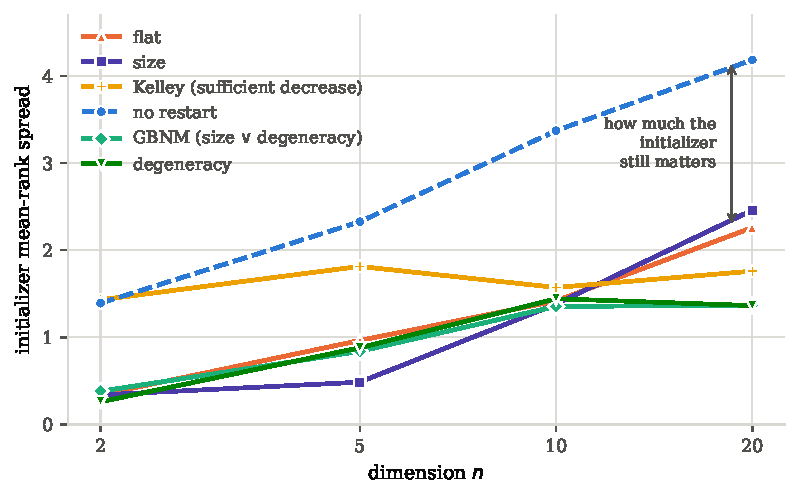
\includegraphics[width=0.78\textwidth]{fig3-spread.pdf}
\caption{Spread in initializer mean rank against dimension. Under a single
descent the choice of initializer matters more and more; any working trigger
holds it far lower, though decreasingly so.}
\label{fig:spread}
\end{figure}

Table~\ref{tab:spread} ranks the seven initializers within each problem. The
main effect is overwhelming in every row (Friedman, $p=2\times10^{-124}$ for
\texttt{none}), so what follows is about magnitude, not power.

\begin{table}[t]
\centering
\caption{Initializer effects. \emph{Top}: mean rank (1 = best of 7), pooled over
dimension---pooled because the \emph{ordering} of initializers is
dimension-stable. \emph{Bottom}: the spread $\max-\min$, which is not, so it is
broken out by dimension.}
\label{tab:spread}
\small
\begin{tabular}{lccccccc}
\toprule
trigger & pfeffer & sp.\ $100\%$ & sp.\ $10\%$ & sp.\ $2\%$ & uniform & gaussian & p.\ basis \\
\midrule
\texttt{none}         & 5.56 & \textbf{2.88} & 3.69 & 4.54 & 3.49 & 4.57 & 3.26 \\
\texttt{progress}     & 4.63 & \textbf{3.19} & 3.86 & 4.37 & 3.84 & 4.57 & 3.55 \\
\texttt{flat}         & 4.25 & \textbf{3.34} & 3.91 & 4.02 & 4.03 & 4.58 & 3.87 \\
\texttt{size}         & 4.17 & \textbf{3.49} & 3.85 & 4.12 & 3.97 & 4.58 & 3.82 \\
\texttt{conditioning} & 3.89 & \textbf{3.58} & 3.84 & 3.90 & 4.17 & 4.54 & 4.07 \\
\texttt{gbnm}         & 3.88 & \textbf{3.65} & 3.86 & 3.88 & 4.17 & 4.54 & 4.01 \\
\bottomrule
\end{tabular}

\vspace{1.2ex}

\begin{tabular}{lcccc}
\toprule
spread by dimension & $n{=}2$ & $n{=}5$ & $n{=}10$ & $n{=}20$ \\
\midrule
\texttt{none}         & 1.39 & 2.32 & 3.37 & 4.18 \\
\texttt{progress}     & 1.43 & 1.81 & 1.57 & 1.76 \\
\texttt{flat}         & 0.34 & 0.96 & 1.42 & 2.26 \\
\texttt{size}         & 0.34 & 0.48 & 1.38 & 2.46 \\
\texttt{conditioning} & 0.26 & 0.88 & 1.44 & 1.36 \\
\texttt{gbnm}         & 0.38 & 0.84 & 1.35 & 1.36 \\
\bottomrule
\end{tabular}
\end{table}

Enabling any trigger collapses the spread---from $2.68$ pooled under a single
descent to $0.89$--$1.24$---and the clearest case is \texttt{pfeffer}, worst of
the seven at $5.56$ under a single descent, reproducing the central claim of
\citet{wessing2019} on his own example, and mid-pack at $3.88$--$4.25$ under any
trigger. \texttt{progress} is intermediate at $1.44$: a local re-seed absorbs
less of the initialization effect than a global one, as one would expect.

The substitution erodes with dimension (Figure~\ref{fig:spread}). Under a single
descent the spread grows monotonically, $1.39 \to 2.32 \to 3.37 \to 4.18$; under
a working trigger it also grows, $0.34 \to 0.48 \to 1.38 \to 2.26$. Restarts
still absorb most of the effect at every dimension, but the absolute residual at
$n=20$ is larger than the entire effect was at $n=2$. One caution on reading
Figure~\ref{fig:spread}: the degeneracy arms show a \emph{low} spread at $n=20$
($1.36$) not because they absorb the initialization effect but because they
perform uniformly badly, which compresses ranks. Spread is only interpretable
for triggers that work.

Across every trigger and dimension the best initializer is the large regular
simplex. We do not rank the two random initializers against each other: BBOB's
box is $[-5,5]^n$ for every problem, so at a fixed algorithm seed
\texttt{uniform} and \texttt{gaussian} draw the \emph{same} initial simplex on
every problem of a given dimension. Their rows therefore rest on one realization
of the initializer, and only the instance-to-instance shift of the optimum
randomizes the comparison. The deterministic initializers---which carry both
claims above---are unaffected, and the trigger comparisons pool over all seven
initializers, so a lucky or unlucky draw enters every trigger arm equally and
cancels.

\subsection{Conditioning does not mediate the effect}

The intuitive account is that initialization sets simplex conditioning,
contraction destroys it, and restarts reset it. The data do not support it. The
Spearman correlation between a run's median Hadamard ratio and its final
objective, computed within (function, dimension, trigger) and pooled, is
$-0.063$, $-0.016$, $-0.031$ and $-0.101$ at $n=2,5,10,20$, with $61\%$, $58\%$,
$56\%$ and $67\%$ of cells negative. We report this because it is the natural
hypothesis, and because it is the most likely reason the degeneracy trigger
underperforms: a criterion measuring a quantity only weakly coupled to progress
cannot identify a good time to restart. The measurement is correlational and
within-cell, and does not establish or exclude a causal role.

\subsection{The dimensional story is not a budget artifact}
\label{sec:budget}

Everything above runs at a budget of $2000n$, and at $n=20$ the no-restart arm
solves only $11.4\%$ of problems, so the dimension might be budget-starved rather
than hard---which would make the trends a statement about the budget instead of
about $n$. We re-ran six arms at $n\in\{10,20\}$ under both $2000n$ and $4000n$,
holding the initializer at the regular simplex.

Quadrupling the effective budget changes nothing material. The mean rank of the
six arms within each problem gives an \emph{identical} ordering at both budgets
and both dimensions (Kendall $\tau = 1.000$), no arm shifting by more than $0.21$
rank; win rates against no-restart move by at most a few points and never change
sign. The one systematic effect is that a larger budget mildly favours the
cheaper triggers---\texttt{size} improves from $75.8\%$ to $89.2\%$ against
no-restart at $n=20$---which sharpens rather than softens the paper's
recommendation.

This run also supplies a comparison the tolerance sweep of
Section~\ref{sec:calibration} could not make, because that sweep contained no
no-restart arm. At its best tolerance the degeneracy trigger beats no-restart on
$84$--$96\%$ of problems at both dimensions and both budgets. So the indictment
in Section~\ref{sec:degeneracy} is emphatically a statement about the published
default: retuned, the criterion is a perfectly serviceable restart trigger that
happens to be no better than testing whether the simplex is small
($39.2\%$--$54.2\%$ against \texttt{size}, indistinguishable from parity at three
of four dimension--budget combinations). At the default it is far worse than
either ($20.0$--$24.2\%$ against \texttt{size}).

\subsection{A caution about unshifted test functions}
\label{sec:caution}

On the five classical analytic functions, over $n\in\{2,5,10\}$, the same
experiment reverses Section~\ref{sec:substitution}: the spread is $3.80$ under a single descent and
$3.60$--$3.82$ under four of five triggers---no substitution at all.

The explanation is that sphere, Rosenbrock, Rastrigin, Ackley and Griewank all
place their optimum at or near the centre of the conventional box, so a
structured simplex built about that centre begins at the answer. Restarts cannot
improve on an initializer that has already won, and the interaction is
suppressed by construction. These functions remain common in the Nelder--Mead
variant literature; for questions about initialization they are not merely weak
but actively misleading, and a shifted, rotated suite is required.

\section{Conclusions}

On \textbf{(Q1)}: restarts substitute for initialization, collapsing the spread
across seven initializers from $2.68$ to $0.89$--$1.24$ and rendering the
\texttt{fminsearch} default unremarkable. The substitution erodes with
dimension, so Wessing's advice is strongest exactly where it is hardest to avoid
needing it. This qualifies \citet{wessing2019} rather than contradicting him, and
reconciles his result with the expensive-objective regime of
\citet{takenaga2023}, where restarts are unaffordable and initialization is
consequently decisive.

On \textbf{(Q2)}: the honest answer is that it depends on $n$, and neither
published detector is a safe default across the range. For $n\le10$ a
simplex-flatness or simplex-size test dominates everything else tested. At
$n=20$ the trivial triggers remain the most consistent, but Kelley's detector
attains the best value on more problems than any other arm, and the degeneracy
test of \citet{luersen2004} has become actively harmful---worse than never
restarting, firing $463$ times per run, and by then accounting for $100\%$ of
GBNM's restarts. A practitioner using GBNM at moderate dimension should disable
Eq.~\eqref{eq:gbnm9} and keep the size test---and Section~\ref{sec:calibration}
shows this is not a tuning failure they can repair: across $40$ orders of
magnitude of $\varepsilon_{s4}$, no setting is significantly better than the size
test at any dimension, and $\varepsilon_{s3}$ is very nearly inert. If a construction that shrinks the
simplex is used, it must be paired with a trigger that does not fire on
smallness---which is exactly what \citet{kelley1999} does.

Three limitations bound these claims. The dimensional trends rest on four
points with one instance seed per problem, and the $n=20$ conclusions are the
least well supported---though Section~\ref{sec:budget} shows they are at least
not an artifact of the evaluation budget. Restart construction has two levels; GBNM's own
probabilistic re-seeding from a kernel density over past search points is not
implemented, and the factorial test of \citet{oneill1971} is not among the
triggers compared. The $f_L$ convention that complicates
Section~\ref{sec:metrics} is discharged rather than merely disclosed: every
headline claim was re-verified against absolute targets recovered from
$f_{\mathrm{opt}}$, and the trends hold under both.

\paragraph{Reproducibility.} Implementation, raw per-run records for all
$43\,050$ runs, the recovered $f_{\mathrm{opt}}$ values, and the analysis scripts
are available at
\url{https://github.com/Mollinetti/NMs/tree/GBNM}. Results were produced with Python 3.14.6, NumPy 2.x,
SciPy 1.x and \texttt{coco-experiment} 2.8.2 on macOS/arm64; every algorithm run
uses seed $101$, and the per-run records carry the initializer, trigger,
construction, tolerances and budget needed to reproduce any single cell.

\bibliographystyle{plainnat}
\bibliography{references}

\end{document}
